Oggi utilizziamo quello che abbiamo imparato dall'equazione di Dirac per risolvere due problemi: introduciamo nell'equazione di Dirac (che descrive il moto di una particella libera) l'interazione con un campo Coulombiano (e elettromagnetico) e studiamo due aspetti. Il primo è il limite a bassa energia infatti vogliamo capire se ritroviamo l'equazione di Schr\"odinger  in realtà con l'equazione di Pauli sarebbe l'equazione scritta con gli spinori bidimensionali (i due stati di spin). E poi vogliamo vedere lo scattering con potenziale coulombiano che è la sezione d'urto di Rutherford sia con particelle di spin 0 (equazioni di Klein-Gordon) e spin $1/2$ (equazione di Dirac)
\section{Interazione elettromagnetica}
Nell'elettrodinamica classica la forza che agisce su una particella carica in moto è data dalla Forza di Lorentz
$$
F = q\mathbf{E} + q\mathbf{v} \times \mathbf{B}
$$
Può essere ricavata (equazione di Hamilton) dall'Hamiltoniana classica
$$
H = \frac{1}{2m}(\mathbf{p} - q\mathbf{A})^2 + qV
$$
Nella meccanica quantistica non relativistica l'interazione elettromagnetica viene introdotta utilizzando l'Hamiltoniana appena introdotta ($\hbar=1$)
$$
H\psi = \left[ \frac{1}{2m}(-i\boldsymbol{\nabla} - q\mathbf{A})^2 + qV \right] \psi = i\frac{\partial}{\partial t}\psi
$$
Inoltre è conveniente riscrivere questa equazione nel modo seguente
$$
\frac{1}{2m} \left[ -i(\boldsymbol{\nabla} - iq\mathbf{A}) \right]^2 \psi = i \left( \frac{\partial}{\partial t} + iqV \right) \psi
$$
Notiamo che si può arrivare all'equazione precedente partendo dall'equazone di Schr\"odinger per una particella libera e fare le sostituzioni
$$
\nabla \to \nabla - iq\mathbf{A} \qquad \frac{\partial}{\partial t} \to \frac{\partial}{\partial t} + iqV
$$
Sviluppando il quadrato nell'Hamiltoniana
$$
H = \frac{1}{2m}(-i\boldsymbol{\nabla} - q\mathbf{A})^2 + qV
$$
$$
(-i\boldsymbol{\nabla} - q\mathbf{A})(-i\boldsymbol{\nabla} - q\mathbf{A})\psi = -\nabla^2\psi + \textcolor{red}{iq\boldsymbol{\nabla} \cdot ({\mathbf{A}\psi})} + iq\mathbf{A} \cdot \boldsymbol{\nabla}\psi + q^2\mathbf{A}^2\psi
$$
$$
= -\nabla^2\psi + \textcolor{red}{iq(\boldsymbol{\nabla} \cdot \mathbf{A})\psi + iq\mathbf{A} \cdot \boldsymbol{\nabla}\psi} + iq\mathbf{A} \cdot \boldsymbol{\nabla}\psi + q^2\mathbf{A}^2\psi
$$
Scegliendo il gauge $\nabla\cdot \mathbf{A}=0$ e trasurando i termini in $q^2$ otteniamo
$$
H = -\frac{1}{2m}\nabla^2 + i\frac{q}{m}\mathbf{A} \cdot \boldsymbol{\nabla} + qV
$$
Applichiamo questa formula al caso di un campo magnetico costante e campo elettrico nullo $V=0 \,\,(i\nabla=\mathbf{p})$
$$
H = -\frac{1}{2m}\nabla^2 - \frac{q}{m}\mathbf{A} \cdot \mathbf{p}
$$
Per un campo magnetico costante $\mathbf{B}$ il potenziale vettore è
$$
\mathbf{A} = -\frac{1}{2}\mathbf{r} \times \mathbf{B}
$$
Introduciamo $\mathbf{A}$ nell'Hamiltoniana
$$
H = -\frac{1}{2m}\nabla^2 + \frac{q}{2m}\mathbf{r} \times \mathbf{B} \cdot \mathbf{p}
$$
Il termine con il campo magnetico può essere trasformato in
$$
(\mathbf{r} \times \mathbf{B}) \cdot \mathbf{p} = \sum_{klm} \varepsilon_{klm} r_l B_m p_k = -\sum_{mlk} \varepsilon_{mlk} B_m r_l p_k = -\mathbf{B} \cdot (\mathbf{r} \times \mathbf{p}) = -\mathbf{B} \cdot \mathbf{L}
$$
$$
H = -\frac{1}{2m}\nabla^2 - \frac{q}{2m}\mathbf{B} \cdot \mathbf{L}
$$
\begin{figure}[h!]
    \centering
    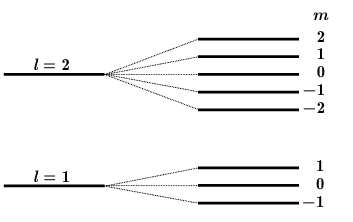
\includegraphics[width=0.4\textwidth]{Lezioni/Lezione 4/mm.png}
    \label{fig:mm}
\end{figure}
L'ultimo termine dell'equazione rappresenta una energia potenziale magnetica. Classicamente è dovuta all'interazione di un momento magnetico generato dal moto associato ad un momento angolare orbitale $\mathbf{L}$. Anche a livello quantistico definiamo pertanto il momento magnetico di una particella dotata di momento angolare $\mathbf{L}$ e la sua energia potenziale
$$
\mu = \frac{q}{2m} \mathbf{L} \qquad U = -\boldsymbol{\mu} \cdot \mathbf{B}
$$
L'esistenza di questo termine di interazione è verificata nella spettroscopia atomica. Infatti, in presenza di un campo magnetico le energie associate agli orbitali atomici di momento angolare $l$ si separano in $(2l+1)$ livelli equidistanti (effetto Zeeman). Inoltre è noto che esiste un ulterior effetto di questo tipo. L'elettrone ha un momento angolare intrinseco $\mathbf{S}=\hbar\sigma/2$ a cui sarebbe associato un momento magnetico $\boldsymbol{\mu}=q\mathbf{S}/2m$ che suddivide ulteriormente i livelli. Tuttavia, nel caso dello spin, per riprodurre i dati sperimentali occorre introdurre un fattore empirico $g$.
$$
\mu_e = \textcolor{red}{g} \frac{q}{2m_e} \mathbf{S} \qquad g=2
$$
Prima di introdurre l'interazione elettromagnetica nell'equazione di Dirac facciamo alcune precisazioni sulle notazioni
$$
\frac{\partial}{\partial x^\mu} \equiv \partial_\mu = \left(\frac{\partial}{\partial x^0}, \nabla\right) \qquad \frac{\partial}{\partial x_\mu} \equiv \partial^\mu = \left(\frac{\partial}{\partial x^0}, \textcolor{red}{-}\nabla\right)
$$
Inoltre il potenziale vettore è
$$
A_\mu = (V(x), \textcolor{red}{-}\mathbf{A}(x)) \qquad A^\mu = (V(x), \mathbf{A}(x))
$$
L'introduzione dell'interazione elettromagnetica viene fatta modificando l'operatore di derivazione (per l'elettrone $q=-|e|$)
$$
\partial_\mu \to \partial_\mu + iqA_\mu
$$
Attenzione: per l'operatore derivazione e il potenziale vettore i segni negativi delle componenti spaziali delle componenti covarianti e controvarianti sono scambiati
$$
\partial_\mu + iqA_\mu = (\partial_0 + iqV, \nabla + iq\mathbf{A}_k) = (\partial_0 + iqV, \nabla \textcolor{red}{-} iqA)
$$
$$
\partial_\mu \to (\partial_0 + iqV, \nabla - iq\mathbf{A})
$$
A questo punto passiamo all'equazione di Dirac
$$
i \frac{\partial}{\partial t} \psi = H_0 \psi = (-i\boldsymbol{\alpha} \cdot \boldsymbol{\nabla} + \beta m)\psi
$$
Con la sostituzione minimale diventa
$$
\partial_\mu \to (\partial_0 + iqV, \nabla - iq\mathbf{A})
$$
$$
i \left( \frac{\partial}{\partial t} + iqV \right) \psi = (-i\boldsymbol{\alpha} \cdot (\boldsymbol{\nabla} - iq\mathbf{A}) + \beta m)\psi
$$
$$
\left( i \frac{\partial}{\partial t} - qV \right) \psi = (\boldsymbol{\alpha} \cdot (-i\boldsymbol{\nabla} - q\mathbf{A}) + \beta m)\psi
$$
$$
i \frac{\partial}{\partial t} \psi = (\boldsymbol{\alpha} \cdot (-i\boldsymbol{\nabla} - q\mathbf{A}) + \beta m + qV)\psi
$$
Utilizzeremo questa formula per lo studio dello scattering da potenziale. Vale la pena isolare il potenziale di interazione
$$
i \frac{\partial}{\partial t} \psi = (H_0 + V_D)\psi \qquad V_D = qV - q\boldsymbol{\alpha} \cdot \mathbf{A}
$$
\section{Limite a bassa energia}
Bisogna prestare attenzione perché è molto istruttivo studiare il limite a bassa energia dell'equazione trovata. Verifichiamo se ci conduce all'equazione di Schr\"odinger con l'interazione elettromagnetica. Per poter confrontare con l'equazione non relativistica occorre tenere conto che l'energia relativistica include la massa a riposo della particelle. Se $H$ è l'Hamiltoniana dobbiamo isolare la massa scrivendo $H=H_1+m$
$$
H = \boldsymbol{\alpha} \cdot (-i\boldsymbol{\nabla} - q\mathbf{A}) + \beta m + qV = \boldsymbol{\alpha} \cdot (-i\boldsymbol{\nabla} - q\mathbf{A}) + \beta m + qV - mI + mI
$$
$$
H_1 = \boldsymbol{\alpha} \cdot (-i\boldsymbol{\nabla} - q\mathbf{A}) + (\beta - I)m + qV
$$
Quindi questo Hamiltoniano è confrontabile con l'Hamiltoniano di Schr\"odinger perché la massa a riposo della particella l'abbiamo isolata. E questo è il primo passo, il secondo passo invece. Inoltre isoliamo la massa a riposo anche nella dipendenza temporale ponendo. Infatti nella meccanica quantistica non relativistica l'energia $E$ di una particella libera è solo la sua energia cinetica. Nella teoria relativistica di Dirac l'energia totale $E$ comprende anche l'energia di massa e riposo. Ricordando che l'evoluzione temporale di uno stato stazionario è dettata dal fattore di fase $e^{-iEt}$. Se scriviamo questo fattore per l'equazione di Dirac nel limite di bassa energia otteniamo:
$$
e^{-iE_\text{dir}t}=e^{-i(m+E_\text{cin})t}=e^{-imt}\cdot e^{-iE_\text{cin}t}
$$
Il termine $e^{-imt}$ è un problema per fare il confronto con l'equazione di Schr\"odinger. Poiché la massa $m$ dell'elettrone (circa $511\,\unit{keV}$) è enorme rispetto alle energie cinetiche non relativistiche. Questo termine rappresenta un'oscillazione ad altissima frequenza che "maschera" la dinamica non relativistica lenta governata da $e^{-E_\text{cin}t}$. Per sbarazzarci di questa oscillazione frenetica ed estrarre la fisica di Schr\"odinger, fattorizziamo esplicitamente l'oscillazione di massa scrivendo la funzione d'onda completa $\Psi(t)$ come:
$$
\Psi(t) = \Psi_0(t) e^{-imt} \qquad \left| \frac{\partial}{\partial t} \Psi_0(t) \right| \ll m
$$
Infatti siamo arrivati al punto chiave: "cosa significa "limite non relativistico?" Significa che l'energia cinetica e l'energia potenziale sono trascurabili rispetto alla massa a riposo ($E_\text{cin}\ll m$ e $|qV|\ll m$). Pertanto, traducendo questa disuguaglianza per la nostra funzione $\Psi_0$ otteniamo matematicamente:
$$
\left| \frac{\partial \Psi_0}{\partial t} \right|\approx E_\text{cin}|\Psi_0|\ll m|\Psi_0|
$$
Quindi $\Psi_0$ lentamente variabile. Inseriamo nell'equazione di Dirac per trovare l'equazione per $\Psi_0$
$$
i \frac{\partial}{\partial t} \Psi(t) = \left( i \frac{\partial}{\partial t}\Psi_0(t) + m \Psi_0(t) \right) e^{-imt} = (H_1 + m) \Psi_0(t) e^{-imt}
$$
$$
i \frac{\partial}{\partial t} \Psi_0 = H_1 \Psi_0
$$
Riepilogando
$$
H_1 = \boldsymbol{\alpha} \cdot (-i\boldsymbol{\nabla} - q\mathbf{A}) + (\beta - I)m + qV \qquad i \frac{\partial}{\partial t} \Psi_0 = H_1 \Psi_0
$$
Utilizziamo la rappresentazione di Pauli-Dirac e la rappresentazione a blocchi dello spinore
$$
\boldsymbol{\alpha} = \begin{pmatrix} 0 & \boldsymbol{\sigma} \\ \boldsymbol{\sigma} & 0 \end{pmatrix} \quad \beta = \begin{pmatrix} I & 0 \\ 0 & -I \end{pmatrix} \quad \Psi = \begin{pmatrix} \psi \\ \phi \end{pmatrix} \quad \beta - I = \begin{pmatrix} 0 & 0 \\ 0 & -2I \end{pmatrix}
$$
Arriviamo al sistema di equazioni
$$
i \frac{\partial}{\partial t} \begin{pmatrix} \psi \\ \phi \end{pmatrix} = \begin{pmatrix} 0 & \boldsymbol{\sigma} \cdot (-i\boldsymbol{\nabla} - q\mathbf{A}) \\ \boldsymbol{\sigma} \cdot (-i\boldsymbol{\nabla} - q\mathbf{A}) & 0 \end{pmatrix} \begin{pmatrix} \psi \\ \phi \end{pmatrix} + qV \begin{pmatrix} \psi \\ \phi \end{pmatrix} - 2m \begin{pmatrix} 0 \\ \phi \end{pmatrix}
$$
$$
\begin{cases}
i \frac{\partial}{\partial t} \psi = \boldsymbol{\sigma} \cdot (-i\boldsymbol{\nabla} - q\mathbf{A}) \phi + qV \psi \\
i \frac{\partial}{\partial t} \phi = \boldsymbol{\sigma} \cdot (-i\boldsymbol{\nabla} - q\mathbf{A}) \psi + qV \phi - 2m\phi
\end{cases}
$$
Considerando la seconda equazione: ricordiamo che $\Psi_0$ varia lentamente, vale a dire che
$$
\left| \frac{\partial}{\partial t} \Psi_0(t) \right| \ll m
$$
Quindi anche le due componenti $\psi$ e $\phi$ variano lentamente
$$
\left| i \frac{\partial}{\partial t} \psi \right| \ll m \qquad \left| i \frac{\partial}{\partial t} \phi \right| \ll m
$$
Abbiamo pertanto (in approssimazione non relativistica) ($qV \ll m$)
$$
i \frac{\partial}{\partial t} \phi = \boldsymbol{\sigma} \cdot (-i\boldsymbol{\nabla} - q\mathbf{A})\psi + qV\phi - 2m\phi
$$
$$
0 = \boldsymbol{\sigma} \cdot (-i\boldsymbol{\nabla} - q\mathbf{A})\psi - 2m\phi
$$
$$
\phi \approx \frac{\boldsymbol{\sigma} \cdot (-i\boldsymbol{\nabla} - q\mathbf{A})}{2m} \psi
$$
Ovviamente questa è una forma approssimata in quanto abbiamo applicato l'approssimazione non relativistica "togliendo" il termine $qV$ e la derivata temporale in quanto molto più piccoli della massa. Introduciamo nella prima equazione
$$
i \frac{\partial}{\partial t} \psi = \boldsymbol{\sigma} \cdot (-i\boldsymbol{\nabla} - q\mathbf{A}) \frac{\boldsymbol{\sigma} \cdot (-i\boldsymbol{\nabla} - q\mathbf{A})}{2m} \psi + qV\psi
$$
Si può verificare che 
$$
[\boldsymbol{\sigma} \cdot (-i\boldsymbol{\nabla} - q\mathbf{A})]^2 = (-i\boldsymbol{\nabla} - q\mathbf{A})^2 - q\boldsymbol{\sigma} \cdot \boldsymbol{\nabla} \times \mathbf{A}
$$
Pertanto l'equazione diventa
$$
i \frac{\partial}{\partial t} \psi = \frac{1}{2m}(-i\boldsymbol{\nabla} - q\mathbf{A})^2 \psi - \frac{q}{2m} \boldsymbol{\sigma} \cdot \mathbf{B} \psi + qV\psi
$$
Questa equazione coincide con l'equazione ottenuta partendo dall'equazione di Schr\"odinger con la sostituzione minimale a meno di un temrine
$$
i \frac{\partial}{\partial t} \psi = \left[ \frac{1}{2m}(-i\boldsymbol{\nabla} - q\mathbf{A})^2 + qV \right] \psi
$$
Il termine in più descrive l'accoppiamento momento magnetico intrinseco dell'elettrone con il campo magnetico
$$
\boldsymbol{\mu} = \textcolor{red}{2} \frac{q}{2m} \frac{\boldsymbol{\sigma}}{2}
$$
Inoltre riproduce perfettamente il fattore giromagnetico $g=2$ che nella teoria non relativistica era stato introdotto empiricamente (e quindi a mano) per far tornare i conti con i dati sperimentali dall'effetto Zeeman anomalo. Quindi questo rappresenta un grande trionfo dell'equazione di Dirac che deriva dall'idea "semplice" di linearizzare l'equazione di Klein-Gordon In conclusione il limite $E\ll m$ dell'equazione di Dirac riproduce l'equazione di Pauli. Il fattore giromagnetico $g=2$ è predetto dalla teoria di Dirac.
\section{Scattering Coulombiano: spin 0}
Come prima applicazione della meccanica quantistica relativistica consideriamo lo scattering Coulombiano per una particella di spin 0. La funzione d'onda della particella obbedisce all'equazione di Klein-Gordon (ha un solo grado di libertà!)
$$
(\partial^\mu \partial_\mu + m^2)\phi(x) = 0
$$
Come nel caso dell'equazione di Dirac l'interazione elettromagnetica viene introdotta utilizzando la sostituzione minimale
$$
\partial_\mu \to \partial_\mu + iqA_\mu
$$
Vediamo come si modifica l'operatore $\partial^\mu\partial_\mu$
$$
\partial^\mu \partial_\mu \phi \to (\partial^\mu + iqA^\mu)(\partial_\mu + iqA_\mu)\phi = \partial^\mu \partial_\mu \phi + iq\partial^\mu(A_\mu\phi) + iqA^\mu \partial_\mu \phi - q^2 A^\mu A_\mu \phi
$$
Inserendo nell'equazione di Klein-Gordon
$$
(\partial^\mu \partial_\mu +\textcolor{red}{ iq\partial^\mu A_\mu + iqA^\mu \partial_\mu - q^2 A^\mu A_\mu} + m^2)\phi = 0
$$
Infatti prima si moltiplica a destra per $\phi$ e dopo si applica $\partial_\mu$ al prodotto $A_\mu\phi$.
$$
(\partial^\mu \partial_\mu + m^2)\phi = -iq(\partial^\mu A_\mu + A^\mu \partial_\mu)\phi + q^2 A^\mu A_\mu \phi \equiv -\hat{V}_{KG}\phi
$$
$$
\hat{V}_{KG} = +iq(\partial^\mu A_\mu + A_\mu \partial^\mu) - q^2 A^\mu A_\mu
$$
A questo punto il problema può essere risolto utilizzando la teoria perturbativa dipendente dal tempo. L'ampiezza di transizione da uno stato iniziale $i$ ad uno stato finale $f$ dovuta ad un potenziale $V$ è data dall'approssimazione (primo ordine)
$$
M_{fi} = -i \int dt \int d^3\mathbf{r} \phi_f^*(\mathbf{r}, t) V(\mathbf{r}, t) \phi_i(\mathbf{r}, t)
$$
$$
M_{fi} = -i \int d^4x \phi_f^*(x) V(x) \phi_i(x)
$$
Utilizziamo il potenziale di Klein-Gordon
$$
\hat{V}_{KG} = +iq(\partial^\mu A_\mu + A_\mu \partial^\mu) - \cancel{q^2 A^\mu A_\mu}
$$
Al primo ordine possiamo trascurare il termine $q^2$
$$
\hat{V}_{KG} \approx +iq(\partial^\mu A_\mu + A_\mu \partial^\mu)
$$
Otteniamo in definitiva
$$
M_{fi} = q \int d^4x \phi_f^*(x) (\partial^\mu A_\mu + A_\mu \partial^\mu) \phi_i(x)
$$
Possiamo elaborare il primo termine integrando per parti per ciascuno dei $4$ integrali
$$
\int d^4x \phi_f^* \partial^\mu (A_\mu \phi_i) = \cancel{[\phi_f^* A_\mu \phi_i]|_{-\infty}^{+\infty}} - \int d^4x (\partial^\mu \phi_f^*) A_\mu \phi_i
$$
Assumiamo che il potenziale $A_\mu$ all'infinito si comporti in modo tale da far tendere a zero il primo termine. L'ampiezza di transizione diventa
$$
M_{fi} = -q \int d^4x (\partial^\mu \phi_f^*) A_\mu \phi_i + q \int d^4x \phi_f^* A_\mu \partial^\mu \phi_i = q \int d^4x [\phi_f^* \partial^\mu \phi_i - (\partial^\mu \phi_f^*) \phi_i] A_\mu
$$
L'espressione dentro parentesi quadra ricorda la corrente di probabilità. Si definisce la corrente di transizione elettromagnetica fra gli stati $i$ e $f$
$$
j_{em}^\mu = iq [\phi_f^* \partial^\mu \phi_i - (\partial^\mu \phi_f^*) \phi_i]
$$
Utilizzando questa corrente l'ampiezza di transizione diventa
$$
M_{fi} = -i \int d^4x j_{em}^\mu(x) A_\mu(x)
$$
Questa espressione è importantissima e apparirà ovunque. Questa formula descrive come è fatto il termine di interazione tra una corrente (particella che si muove) e un potenziale. A questo punto utilizziamo due soluzioni con energia positiva dell'equazione di KG: ad esempio un elettrone con carica $q=-e$ $e>0$.
\begin{itemize}
    \item Un'onda piana per lo stato iniziale $\phi_i(x)=e^{-ip_i\cdot x}$
    \item Un'onda piana per lo stato finale $\phi_f(x)=e^{-ip_f\cdot x}$
\end{itemize}
Abbiamo scelto la costante di normalizzazione $N=1$. Inserendo nella corrente di transizione
$$
j_{em}^\mu = -ie[\phi_f^*(\partial^\mu \phi_i) - (\partial^\mu \phi_f^*)\phi_i] = -ie[e^{ip_f \cdot x}(-ip_i^\mu)e^{-ip_i \cdot x} - (-ip_f^\mu)e^{ip_f \cdot x}e^{-ip_i \cdot x}]
$$
$$
j_{em}^\mu(x) = -e(p_f^\mu + p_i^\mu)e^{-i(p_i - p_f) \cdot x}
$$
Otteniamo pertanto
$$
M_{fi} = -i \int d^4x j_{em}^\mu(x) A_\mu(x) = i \int d^4x e(p_f^\mu + p_i^\mu) e^{-i(p_i - p_f) \cdot x} A_\mu(x)
$$
$$
M_{fi} = ie(p_f^\mu + p_i^\mu) \int d^4x e^{-i(p_i - p_f) \cdot x} A_\mu(x)
$$
Consideriamo infine un potenziale Coulombiano
$$
A_\mu(x) = (A_0, \mathbf{0}) \qquad A_0(x) = A_0(\mathbf{r}) = \frac{Ze}{4\pi\varepsilon_0 r}
$$
$$
M_{fi} = ie(p_i^0 + p_f^0) \int d^4x e^{-i(p_i - p_f) \cdot x} A_0(x)
$$
L'ampiezza di transizione diventa pertanto
$$
M_{fi} = ie(E_i + E_f) \int e^{-i(E_i - E_f)t} dt \int d^3\mathbf{r} e^{-i(\mathbf{p}_f - \mathbf{p}_i) \cdot \mathbf{r}} A_0(r)
$$
I due integrali sono indipendenti. L'integrale rispetto al tempo conduce ad una funzione $\delta$
$$
\int e^{-i(E_i - E_f)t} dt = 2\pi\delta(E_i - E_f)
$$
Il secondo integrale è la trasformata di Fourier del potenziale di Coulomb. Si calcola facilmente come limite per $m\to0$ del potenziale di Yukawa
$$
\mathbf{q} = \mathbf{p}_f - \mathbf{p}_i \qquad \int d^3\mathbf{r} e^{-i(\mathbf{p}_f - \mathbf{p}_i) \cdot \mathbf{r}} A_0(\mathbf{r}) = \frac{Ze}{\varepsilon_0} \frac{1}{|\mathbf{q}|^2}
$$
Tenendo conto che
$$
\delta(E_i - E_f) \to E_i = E_f
$$
E inserendo nell'ampiezza di transizione
$$
M_{fi} = ie(E_i + E_f) 2\pi\delta(E_i - E_f) \frac{Ze}{\varepsilon_0} \frac{1}{|\mathbf{q}|^2} = i\pi 4E_i \delta(E_i - E_f) \frac{Ze^2}{\varepsilon_0} \frac{1}{|\mathbf{q}|^2}
$$
$$
\alpha = \frac{e^2}{4\pi\varepsilon_0 \hbar c}
$$
$$
M_{fi} = i4\pi^2 Z\alpha \frac{4E_i}{|\mathbf{q}|^2} \delta(E_i - E_f)
$$
Sempre nel sistema di unità naturali ($\hbar=c=1$). Nella teoria perturbativa dipendente dal tempo la sezione d'urto è data dalla regola d'oro di Fermi
$$
d\sigma = \frac{\dot{P}}{\Phi}
$$
La quantità $\Phi$ è il flusso delle particelle mentre la quantità $\dot{P}$ è la probabilità di transizione per unità di tepo e si calcola a partire dall'elemento di matrice $M_{fi}$
$$
M_{fi} = (2\pi i)\delta(E_f - E_i) V_{fi} \qquad \dot{P} = 2\pi |V_{fi}|^2 \rho(E_f)
$$
In cui $E_i=E_f$. La quantità $\rho(E_f)$ è la densità degli stati. L'elemento di matrice ridotto $V_{fi}$ viene introdotto per isolare la funzione $\delta$. Però il modulo della funzione $\delta$ non è definita. Viene calcolata con un opportuno processo di limite. Ricordando il risultato della diapositiva precedente
$$
M_{fi} = i4\pi^2 Z\alpha \frac{4E_i}{|\mathbf{q}|^2} \delta(E_i - E_f)
$$
Isoliamo l'elemento di matrice ridotto
$$
V_{fi} = 2\pi Z\alpha \frac{4E_i}{|\mathbf{q}|^2}
$$
Vediamo adesso alla densità degli stati: ad una energia $E_f$ corrispondono tutti gli stati con momento $\mathbf{p}_f$. Il numero di stati nell'elemento $d^3\mathbf{p}_f$ dello spazio delle fasi è
$$
dN = \frac{d^3\mathbf{p}_f}{(2\pi)^3 2E_f}
$$
Il fattore $2E_f$ nel denominatore è stato introdotto in modo da rendere $dN$ invariante per trasformazioni di Lorentz. Uguagliando al numero di stati nell'intervallo $dE_f$
$$
\rho(E_f)dE_f = dN = \frac{d^3\mathbf{p}_f}{(2\pi)^3 2E_f}
$$
Calcoliamo esplicitamente $dN$ in funzione di $dE_f$. Utilizzando le coordinate sferiche per $\mathbf{p}_f$
$$
\frac{d^3\mathbf{p}_f}{(2\pi)^3 2E_f} = \frac{|\mathbf{p}_f|^2 d|\mathbf{p}_f| d\Omega}{(2\pi)^3 2E_f} = \frac{|\mathbf{p}_f| E_f dE_f d\Omega}{(2\pi)^3 2E_f}
$$
Avendo utilizzado:
$$
E^2 - m^2 = |\mathbf{p}|^2 \qquad \Longrightarrow \qquad 2EdE = 2|\mathbf{p}|d|\mathbf{p}|
$$
In conclusione
$$
\rho(E_f) = \frac{dN}{dE_f} = \frac{|\mathbf{p}_f| d\Omega}{2(2\pi)^3}
$$
\begin{figure}[h!]
    \centering
    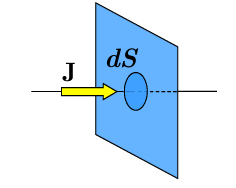
\includegraphics[width=0.4\textwidth]{Lezioni/Lezione 4/jj.png}
    \label{fig:jj}
\end{figure}
Per finire il flusso $\Phi$: le probabilità calcolate sono relative al flusso della corrente incidente (particelle incidenti). La corrente dipende dalla normalizzazione delle funzioni d'onda
$$
dN = |\mathbf{J}| dS \qquad \Phi = \frac{dN}{dS} = |\mathbf{J}|
$$
Occorre tenere conto della normalizzazione degli stati infatti abbiamo visto che per soluzione dell'equazione di KG utilizzate ($N=1$) si ha
$$
\Phi = |\mathbf{J}| = 2|\mathbf{p}_i|
$$
Abbiamo pertanto
\begin{align*}
d\sigma &= \frac{\dot{P}}{\Phi} = \frac{2\pi |V_{fi}|^2}{\Phi} \rho(E_f) = 2\pi \frac{1}{2|\mathbf{p}_i|} \left| 2\pi Z\alpha \frac{4E_i}{|\mathbf{q}|^2} \right|^2 \frac{|\mathbf{p}_f| d\Omega}{2(2\pi)^3} \\
&= (2\pi)^3 (Z\alpha)^2 \frac{(4E_i)^2}{|\mathbf{q}|^4} \frac{|\mathbf{p}_f|}{4(2\pi)^3} \frac{d\Omega}{|\mathbf{p}_i|} = (Z\alpha)^2 \frac{4E_i^2}{|\mathbf{q}|^4} d\Omega
\end{align*}
Dove nell'ultimo passaggio abbiamo imposto che siamo nel caso di scattering elastico $|\mathbf{p}_i|=|\mathbf{p}_f|$. In conclusione otteniamo la sezione d'urto differenziale per lo scattering di una particella di spin $0$ da un potenziale Coulombiano è:
$$
\frac{d\sigma}{d\Omega} = (Z\alpha)^2 \frac{E_i^2}{|\mathbf{q}|^4}
$$
Un ultima elaborazione per sostituire l'angolo di diffusione al momento trasferito
\begin{figure}[h!]
    \centering
    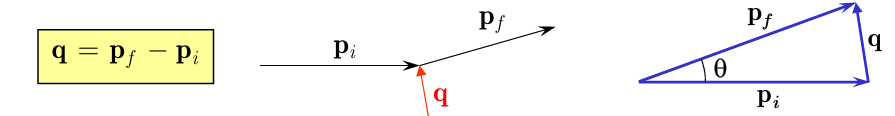
\includegraphics[width=0.7\textwidth]{Lezioni/Lezione 4/pp.png}
    \label{fig:pp}
\end{figure}
Otteniamo pertanto
$$
\mathbf{q}^2=\mathbf{p}^2_f+\mathbf{p}_i^2-2|\mathbf{p}_f||\mathbf{p}_i|\cos{\theta} \qquad \mathbf{q}^2=2\mathbf{p}^2\left(1-\cos{\theta}\right) \qquad \mathbf{q}^2=4\mathbf{p}^2\sin^2{\frac{\theta}{2}}
$$
La sezione d'urto diventa pertanto
$$
\frac{d\sigma}{d\Omega} = (Z\alpha)^2 \frac{E_i^2}{4|\mathbf{p}|^4 \sin^4 \frac{\theta}{2}}
$$
Da confrontare con la formula non relativistica
$$
\frac{d\sigma}{d\Omega} = (Z\alpha)^2 \frac{1}{(4E_K)^2 \sin^4 \frac{\theta}{2}}
$$
\section{Scattering Coulombiano: spin 1/2}
Calcoliamo adesso la sezione d'urto per particelle di spin $\frac{1}{2}$. Il calcolo segue le linee precedenti seguite per le particelle di spin 0. Occorre però utilizzare gli spinori e il potenziale di Dirac. Ricordiamo che l'introduzione dell'interazione elettromagnetica tramite l'accoppiamento minimale aveva condotto all'equazione di Dirac con il potenziale $V_D$
$$
i \frac{\partial}{\partial t} \psi = (H_0 + V_D) \psi \qquad V_D = qV - q\boldsymbol{\alpha} \cdot \mathbf{A}
$$
Come nel caso dell'equazione di KG utilizziamo la teoria perturbativa dipendente dal tempo. L'elemento di matrice diventa
$$
M_{fi} = -i \int dt \int d^3\mathbf{r} \psi_f^\dagger(\mathbf{r}, t) \hat{V}_D(\mathbf{r}, t) \psi_i(\mathbf{r}, t)
$$
Utilizziamo due soluzioni con energia positiva:
\begin{itemize}
    \item Uno stato iniziale con momento $\mathbf{p}_i$ e spin $s_i$ 
    $$
    \psi_i(x) = u(\mathbf{p}_i, s_i) e^{-ip_i \cdot x}
    $$
    \item Uno stato finale con momento $\mathbf{p}_f$ e spin $s_f$ 
    $$
    \psi_f(x) = u(\mathbf{p}_f, s_f) e^{-ip_f \cdot x}
    $$
\end{itemize}
Inserendo nell'elemento di matrice 
$$
M_{fi} = -i \int u_f^\dagger(\mathbf{p}_f, s_f) \hat{V}_D(x) u_i(\mathbf{p}_i, s_i) e^{-i(p_i - p_f) \cdot x} d^4x
$$
Introduciamo $I=\gamma^0\gamma^0$ fra lo spinore $u_f$ e il potenziale $V_D$ e semplifichiamo la notazione: $u_i(p_i,s_i)=u_i$, etc.
$$
M_{fi} = -i \int u_f^\dagger \gamma^0 \gamma^0 \hat{V}_D(x) u_i e^{-i(p_i-p_f) \cdot x} d^4x
$$
Elaboriamo l'respessione del potenziale
$$
V_D=qV-q\boldsymbol{\alpha}\cdot\mathbf{A}
$$
$$
\gamma^0 V_D = q\gamma^0 A_0 - q\gamma^0 \boldsymbol{\alpha} \cdot \mathbf{A} = q\gamma^0 A_0 - q\boldsymbol{\gamma} \cdot \mathbf{A} = q\gamma^\mu A_\mu
$$
$$
\gamma^0 \hat{V}_D = q\gamma^\mu A_\mu
$$
Inserendo nell'elemento di matrice
$$
M_{fi} = -iq \int \overline{u}_f \gamma^\mu u_i A_\mu e^{-i(p_i-p_f) \cdot x} d^4x
$$
Come nel caso di KG è interessante introdurre la corrente di transizione elettromagnetica
$$
j_{em}^\mu(x) = q\overline{\psi}_f(x)\gamma^\mu \psi_i(x) = q\overline{u}_f \gamma^\mu u_i e^{-i(p_i-p_f) \cdot x}
$$
$$
M_{fi} = -i \int j_{em}^\mu(x) A_\mu(x) d^4x
$$
Per finire, consideriamo un elettrone ($q=-e$ $e>0$) in un campo Coulombiano statico
$$
M_{fi} = ie\overline{u}_f \gamma^\mu u_i \int A_\mu e^{-i(p_i-p_f) \cdot x} d^4x \qquad A_\mu(x) = (A_0, \mathbf{0}) \qquad A_0(x) = A_0(\mathbf{r}) = \frac{Ze}{4\pi\epsilon_0 r}
$$
Confrontando con il calcolo per la particella di spin $0$
$$
M_{fi} = ie(p_i^0 + p_f^0) \int d^4x e^{-i(p_i-p_f) \cdot x} A_0(x)
$$
Il calcolo dell'integrale è identico al caso della particella di spin $0$ solo che al termine $2E_i=\left(p^0_i+p^0_f\right)$ sostituiamo $\overline{u}_f\gamma^0u_i=u_f^\dagger u_i$. Introducendo anche in questo caso l'elemento di matrice ridotto otteniamo
$$
V_{fi} = 2\pi Z\alpha \frac{2}{|\mathbf{q}|^2} u_f^\dagger u_i
$$
$$
d\sigma = \frac{\dot{P}}{\Phi} = \frac{2\pi |V_{fi}|^2}{\textcolor{red}{\Phi}} \textcolor{blue}{\rho(E_f)} = \textcolor{red}{\frac{1}{2|\mathbf{p}_i|}} \left| 2\pi Z\alpha \frac{2}{|\mathbf{q}|^2} \right|^2 |u_f^\dagger u_i|^2 \textcolor{blue}{\frac{|\mathbf{p}_f| d\Omega}{2(2\pi)^3}} = (Z\alpha)^2 \frac{|u_f^\dagger u_i|^2}{|\mathbf{q}|^4} d\Omega
$$
$$
\frac{d\sigma}{d\Omega} = (Z\alpha)^2 \frac{|u_f^\dagger u_i|^2}{|\mathbf{q}|^4}
$$
Gli stati iniziale e finale possono avere ciascuno due stati di polarizzazione: indicandoli convenzionalmente $+$ o $-$ otteniamo 4 sezioni d'urto
$$
d\sigma_{++} \sim |u_+^\dagger u_+|^2 \qquad d\sigma_{-+} \sim |u_+^\dagger u_-|^2 \qquad d\sigma_{+-} \sim |u_-^\dagger u_+|^2 \qquad d\sigma_{--} \sim |u_-^\dagger u_-|^2
$$
Supponiamo di distinguere (misurare) la polarizzazione dello stato finale. Se non utilizziamo un fascio polarizzato la sezione d'urto si ottiene mediando le due sezioni d'urto con polarizzazione dello stato iniziale $+$ e $-$. Quindi noi stiamo isolando una data polarizzazione dello stato finale e diciamo che la sezione d'urto è dato dal valore mediato delle due sezioni d'urto che hanno polarizzazione iniziale $+$ e $-$ (sommo e divido per $2$).
$$
d\sigma_{+} = \frac{1}{2} (d\sigma_{+\textcolor{red}{+}} + d\sigma_{+\textcolor{red}{-}}) \sim \frac{1}{2} (|u_+^\dagger u_{\textcolor{red}{+}}|^2 + |u_+^\dagger u_{\textcolor{red}{-}}|^2)
$$
$$
d\sigma_{-} = \frac{1}{2} (d\sigma_{-\textcolor{red}{+}} + d\sigma_{-\textcolor{red}{-}}) \sim \frac{1}{2} (|u_-^\dagger u_{\textcolor{red}{+}}|^2 + |u_-^\dagger u_{\textcolor{red}{-}}|^2)
$$
Il fattore $\frac{1}{2}$ deriva dal fatto che è una media. Se non si osserva neppure la polarizzazione nello stato finale la sezione d'urto misurata è la somma $d\sigma=d\sigma_++d\sigma_-$ (somma! NON media). Occorre pertanto calcolare
$$
C = \frac{1}{2} [|u_+^\dagger u_+|^2 + |u_+^\dagger u_-|^2 + |u_-^\dagger u_+|^2 + |u_-^\dagger u_-|^2]
$$
L'espressione $C$ può essere calcolata utilizzando, ad esempio, la forma esplicita degli spinori nella rappresentazione di Dirac. Il calcolo di "forza bruta" porta al risultato
$$
C = 4E_i^2 \left( 1 - \beta^2 \sin^2 \frac{\theta}{2} \right)
$$
Introducendo nella formula della sezione d'urto
$$
\frac{d\overline{\sigma}}{d\Omega} = \sum_{k=\pm, l=\pm} \frac{d\sigma_{kl}}{d\Omega} = (Z\alpha)^2 \frac{\sum_{k=\pm, l=\pm} |u_k^\dagger u_l|^2}{16 |\mathbf{p}|^4 \sin^4 \frac{\theta}{2}}
$$
Otteniao finalmente
$$
\frac{d\overline{\sigma}}{d\Omega} = (Z\alpha)^2 \frac{E_i^2}{4|\mathbf{p}|^4 \sin^4 \frac{\theta}{2}} \left( 1 - \beta^2 \sin^2 \frac{\theta}{2} \right)
$$
Osserviamo che la differenza con la particella di spin 0 è data dal fattore 
$$
\left( 1 - \beta^2 \sin^2 \frac{\theta}{2} \right)
$$
Quindi lo spin della particella introduce questo fattore. Nel limite non relativistico $\beta\to 0$ tutto questo termine sparisce e le due sezioni d'urto diventano uguali. Quindi il fatto che una particella abbia o non abbia spin in uno scattering coulombiano non fa differenza. Non ci sorprende perché l'interazione a bassa energia è un'interazione magnetica ma lo spin nel limite non relativistico non interagisce con il campo magnetico. Quindi nel limite a bassa energia le sezioni d'urto tra  scattering con spin e senza spin sono uguali. E sperimentalmente lo sono!
Perché c'è proprio questa dipendenza? In maniera intuitiva nel sistema di riposo dell'elettrone allora questo interagisce solo in maniera magnetica non con campo elettrico. Ma il campo di Coulomb come diventa questo campo? Vedo il nucleo che viene verso di me e acquista un campo magnetico. Quindi ho interazione magnetica tra spin e campo magnetico e quindi deve esserci questa dipendenza della velocità. Più vado veloce più intenso è il campo magnetico.
Il fattore diventa importante per $\beta\to1$: interazione di tipo magnetico. Nel sistema di riposo dell'elettrone al campo elettrico si aggiunge un campo magnetico come effetto relativistico. La sezione d'urto tende a zero per $\beta\to1$ e $\theta\to\pi$ vedremo che è dovuto alla conservazione del momento angolare.